\documentclass[20pt]{extarticle}

\usepackage[paperwidth=841mm,paperheight=1189mm,margin=18mm]{geometry}
\usepackage{lmodern}
\usepackage{graphicx}
\usepackage{xcolor}
\usepackage{booktabs}
\usepackage{tabularx}
\usepackage{array}
\usepackage{enumitem}
\usepackage{amsmath}
\usepackage{pgfplots}
\usepackage{qrcode}
\usepackage{hyperref}
\usepackage{ragged2e}

\pgfplotsset{compat=1.18}
\pagestyle{empty}
\setlength{\parindent}{0pt}
\setlength{\parskip}{2.5mm}
\renewcommand{\familydefault}{\rmdefault}

\definecolor{Night}{HTML}{071017}
\definecolor{Paper}{HTML}{F1F0E8}
\definecolor{Muted}{HTML}{AAB8BF}
\definecolor{Rule}{HTML}{3B515E}
\definecolor{Evidence}{HTML}{56B4E9}
\definecolor{Catalogue}{HTML}{B8E038}
\definecolor{Problem}{HTML}{E69F00}
\pagecolor{Night}
\color{Paper}

\hypersetup{
  colorlinks=false,
  pdfborder={0 0 0},
  pdftitle={The Perturbation Catalogue — An Integrated Resource for Exploring the Impact of Genetic Perturbations},
  pdfauthor={Kirill Tsukanov, Aleksandr Zakirov, Alexey Sokolov, Mallory Freeberg}
}

\newcommand{\sectiontitle}[2]{%
  \vspace{3mm}%
  {\color{#1}\rule{\linewidth}{1.8mm}}\par\vspace{2mm}%
  {\fontsize{44}{50}\selectfont\bfseries #2}\par\vspace{4mm}}
\newcommand{\bodycopy}{\fontsize{29}{36}\selectfont}
\newcommand{\smallcopy}{\fontsize{24}{30}\selectfont}
\newcommand{\tinycopy}{\fontsize{18}{22}\selectfont}
\newcommand{\subhead}[2]{{\fontsize{32}{38}\selectfont\bfseries\color{#1}#2}\par\vspace{2mm}}
\newcommand{\bignumber}[2]{{\fontsize{46}{50}\selectfont\bfseries\color{#1}#2}}
\newcolumntype{Y}{>{\RaggedRight\arraybackslash}X}

\begin{document}
\RaggedRight

% Title -----------------------------------------------------------------------
{\fontsize{64}{69}\selectfont\bfseries The Perturbation Catalogue}\par
\vspace{1mm}
{\fontsize{43}{48}\selectfont\bfseries
An Integrated Resource for Exploring the Impact of Genetic Perturbations}\par

\vspace{5mm}
{\fontsize{23}{28}\selectfont
Kirill Tsukanov \textbullet\ Aleksandr Zakirov \textbullet\ Alexey Sokolov \textbullet\ Mallory Freeberg\
\color{Muted}EMBL European Bioinformatics Institute, Wellcome Genome Campus, Hinxton, United Kingdom}

\vspace{7mm}

% 1. Growth and fragmentation --------------------------------------------------
% Europe PMC query used for the chart (run separately for each year, 2015--2025):
% (TITLE_ABS:"CRISPR screen" OR TITLE_ABS:"CRISPR screening" OR TITLE_ABS:"Perturb-seq"
%  OR TITLE_ABS:"deep mutational scanning" OR TITLE_ABS:"multiplexed assay of variant effect")
% AND FIRST_PDATE:[YYYY-01-01 TO YYYY-12-31]
\sectiontitle{Evidence}{Perturbation evidence is growing faster than it can be organised}
\noindent
\begin{minipage}[t]{0.59\linewidth}
  \vspace{0pt}
  {\fontsize{27}{32}\selectfont\bfseries Publications per year: \textcolor{Evidence}{18 $\longrightarrow$ 655} in a decade}\par
  \vspace{1mm}
  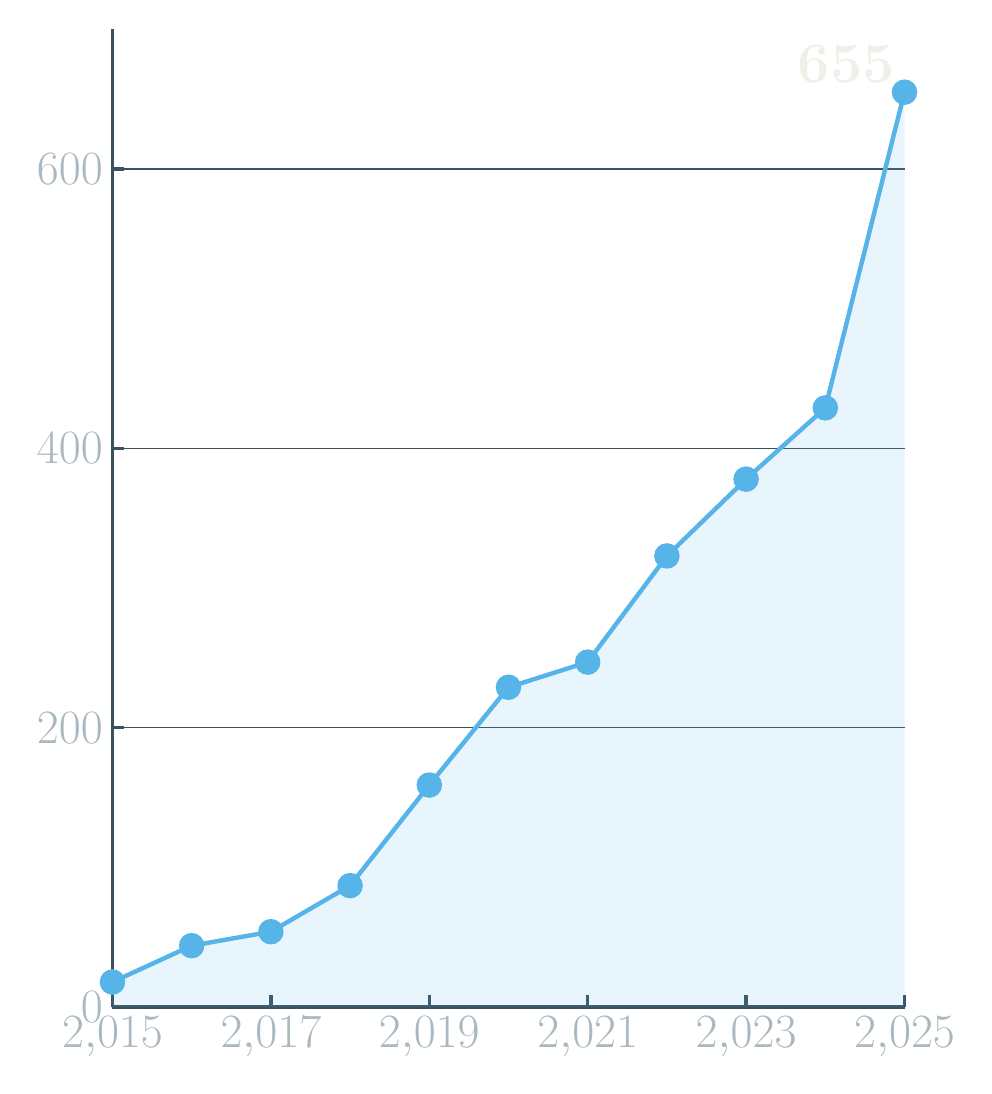
\begin{tikzpicture}
    \begin{axis}[
      width=0.96\linewidth,
      height=140mm,
      xmin=2015, xmax=2025,
      ymin=0, ymax=700,
      xtick={2015,2017,2019,2021,2023,2025},
      ytick={0,200,400,600},
      axis line style={draw=Rule,very thick},
      tick style={draw=Rule,very thick},
      tick label style={font=\fontsize{18}{21}\selectfont,color=Muted},
      xmajorgrids=false,
      ymajorgrids=true,
      major grid style={draw=Rule},
      axis x line*=bottom,
      axis y line*=left,
      clip=false]
      \addplot[draw=none,fill=Evidence,fill opacity=.13]
        coordinates {(2015,18)(2016,44)(2017,54)(2018,87)(2019,159)(2020,229)(2021,247)(2022,323)(2023,378)(2024,429)(2025,655)} \closedcycle;
      \addplot[color=Evidence,ultra thick,mark=*,mark size=3.8pt]
        coordinates {(2015,18)(2016,44)(2017,54)(2018,87)(2019,159)(2020,229)(2021,247)(2022,323)(2023,378)(2024,429)(2025,655)};
      \node[anchor=south east,font=\fontsize{21}{24}\selectfont\bfseries,color=Paper]
        at (axis cs:2025,655) {655};
    \end{axis}
  \end{tikzpicture}

  {\tinycopy\color{Muted}
  Europe PMC yearly publication counts for title/abstract mentions of CRISPR screens, Perturb-Seq,
  deep mutational scanning or multiplexed assays of variant effect; snapshot 24 August 2026.}
\end{minipage}\hfill
\begin{minipage}[t]{0.37\linewidth}
  \vspace{0pt}
  \bignumber{Evidence}{36$\times$}\par
  {\bodycopy more papers per year than in 2015.}

  \vspace{7mm}
  \bignumber{Evidence}{$>$2.5 million}\par
  {\bodycopy cells profiled in a single genome-scale Perturb-Seq study.}
  {\tinycopy\color{Muted}Replogle et al., \emph{Cell} 2022; doi:10.1016/j.cell.2022.05.013.}

  \vspace{7mm}
  {\bodycopy
  This evidence is exceptionally rich, but studies arrive with different repositories, identifiers, metadata depth,
  score semantics, gene annotations and processing choices. The result is abundance without straightforward reuse.}
\end{minipage}

\vfill

% 2. Integration ---------------------------------------------------------------
\sectiontitle{Catalogue}{The Catalogue turns scattered studies into one coherent resource}
{\smallcopy
\renewcommand{\arraystretch}{1.2}
\setlength{\tabcolsep}{4mm}
\begin{tabularx}{\linewidth}{@{}Y >{\centering\arraybackslash}p{22mm} Y >{\centering\arraybackslash}p{22mm} Y@{}}
  \subhead{Problem}{What arrives} && \subhead{Catalogue}{What the Catalogue standardises} && \subhead{Evidence}{What users can retrieve} \\
  Papers, supplements, repository records, matrices and raw sequencing files
  & {\fontsize{35}{38}\selectfont\color{Muted}$\longrightarrow$} &
  One validated metadata schema; Ensembl gene identity; ontology-aligned context; modality-appropriate analysis; explicit provenance
  & {\fontsize{35}{38}\selectfont\color{Muted}$\longrightarrow$} &
  Search by target or dataset; REST API; JSON metadata; complete CSV and Parquet files; interactive modality views \\
  \addlinespace[4mm]
  Author-specific formats and processing decisions
  && BigQuery and dbt harmonise analytical tables; Elastic and PostgreSQL serve search and results
  && The same identifiers, metadata contract and access methods across modalities
\end{tabularx}}

\vspace{3mm}
{\bodycopy
The schema preserves real biological differences—model system, assay, perturbation mechanism, time point and readout—while
removing avoidable technical friction. For selected Perturb-Seq studies, raw FASTQ is reprocessed through a shared workflow
covering counts, guide assignment, quality control, differential expression and Hallmark gene-set enrichment.}

\vfill

% 3. Current state -------------------------------------------------------------
\sectiontitle{Evidence}{Today, 1,237 datasets span three complementary modalities}
\noindent
\begin{minipage}[t]{0.158\linewidth}\bignumber{Catalogue}{1,237}\par{\smallcopy datasets}\end{minipage}\hfill
\begin{minipage}[t]{0.158\linewidth}\bignumber{Catalogue}{19,235}\par{\smallcopy human targets}\end{minipage}\hfill
\begin{minipage}[t]{0.158\linewidth}\bignumber{Catalogue}{36}\par{\smallcopy tissues}\end{minipage}\hfill
\begin{minipage}[t]{0.158\linewidth}\bignumber{Catalogue}{34}\par{\smallcopy cell types}\end{minipage}\hfill
\begin{minipage}[t]{0.158\linewidth}\bignumber{Catalogue}{1,200}\par{\smallcopy cell lines}\end{minipage}\hfill
\begin{minipage}[t]{0.158\linewidth}\bignumber{Catalogue}{169}\par{\smallcopy diseases}\end{minipage}

\vspace{7mm}
\noindent
\begin{minipage}[t]{0.44\linewidth}
  \subhead{Evidence}{CRISPR screens — 1,201 datasets}
  {\bodycopy Gene-level phenotype and fitness scores, harmonised significant hits and rich experimental context.}

  \vspace{4mm}
  \subhead{Evidence}{Perturb-Seq — 26 datasets}
  {\bodycopy Single-cell transcriptomic responses, including differential expression and pathway enrichment. Five datasets
  have been reprocessed from raw FASTQ through the shared pipeline.}

  \vspace{4mm}
  \subhead{Evidence}{MAVE — 10 datasets}
  {\bodycopy Variant-level functional measurements across protein sequence, with searchable scores and effect heatmaps.}

  \vspace{5mm}
  {\smallcopy\color{Muted}Production snapshot: 24 August 2026. All modalities use normalised Ensembl gene IDs.}
\end{minipage}\hfill
\begin{minipage}[t]{0.52\linewidth}
  \vspace{1mm}
  {\setlength{\fboxsep}{2mm}\fcolorbox{Rule}{Paper}{%
    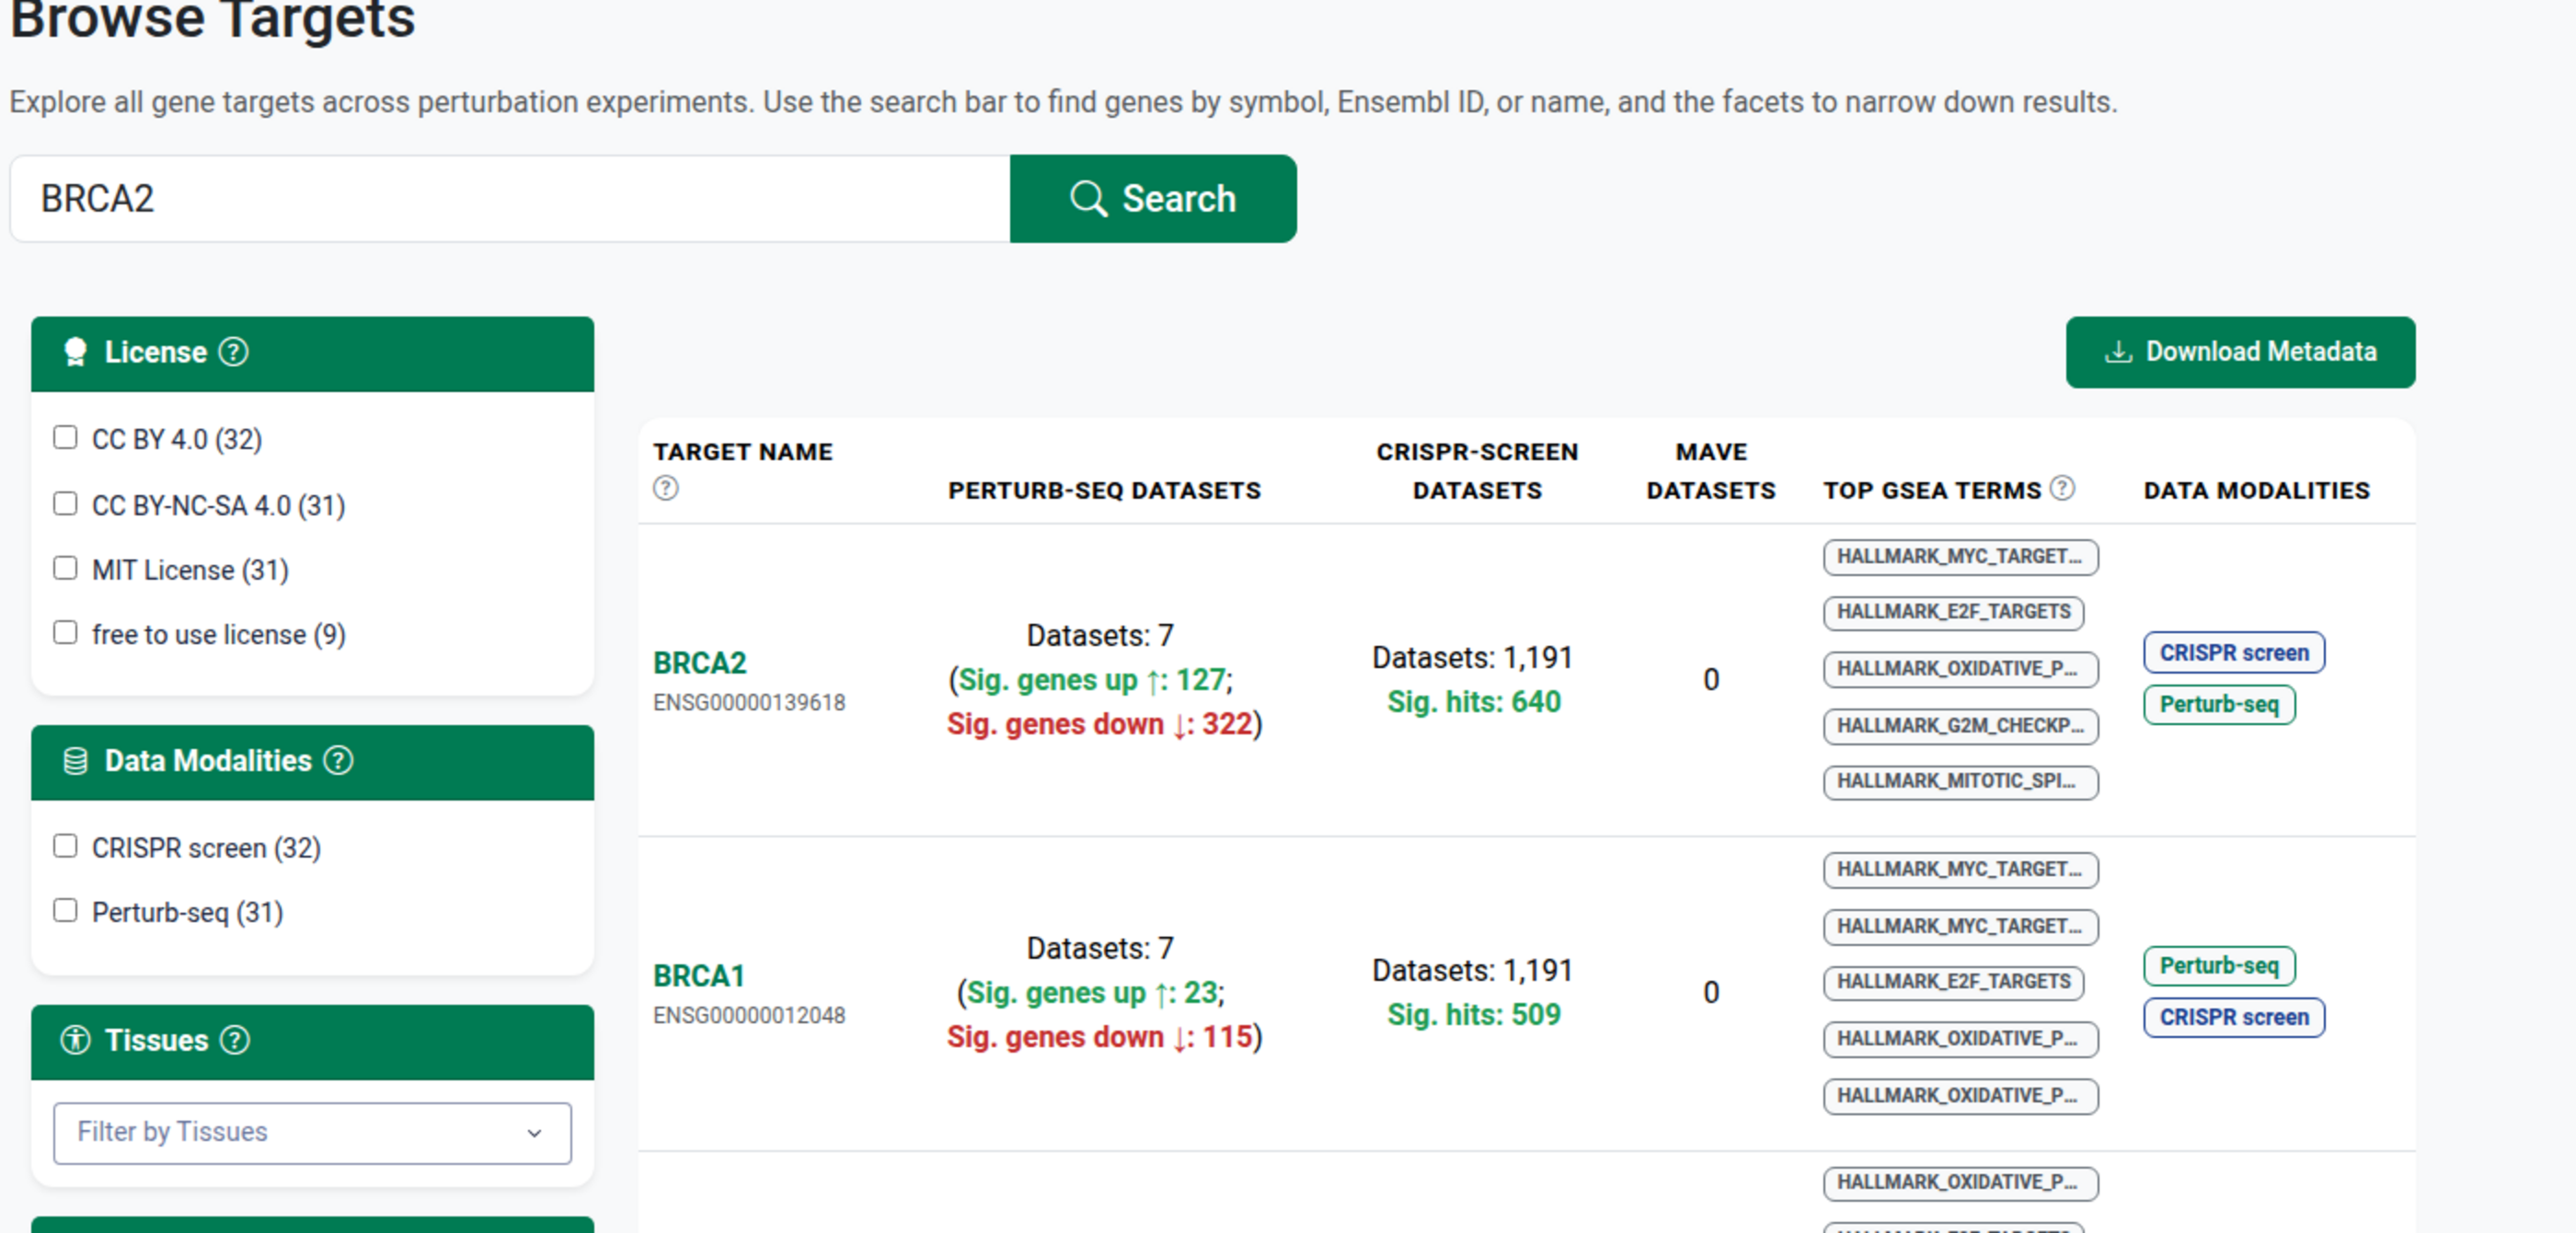
\includegraphics[width=0.978\linewidth]{assets/target-search.png}}}
  {\tinycopy\color{Muted}
  The live BRCA2 target view brings modality coverage, contributing datasets, significant effects and enriched pathways together.}
\end{minipage}

\vfill

% 4. Roadmap -------------------------------------------------------------------
\sectiontitle{Catalogue}{Next, we will make integration continuous and reanalysis broader}
\noindent
\begin{minipage}[t]{0.31\linewidth}
  \subhead{Catalogue}{Curate faster, keep human judgement}
  {\bodycopy AI-assisted extraction will draft structured metadata from studies and repositories. Curators will review
  biological interpretation, resolve ambiguity and validate ontology mappings before release.}
\end{minipage}\hfill
\begin{minipage}[t]{0.31\linewidth}
  \subhead{Catalogue}{Reanalyse more, measure quality}
  {\bodycopy We will extend kit and experimental-design support, develop author-independent quality metrics and broaden
  modality-appropriate reanalysis beyond the first five Perturb-Seq datasets.}
\end{minipage}\hfill
\begin{minipage}[t]{0.31\linewidth}
  \subhead{Catalogue}{Release predictably, preserve provenance}
  {\bodycopy Periodic, versioned releases will make additions and analytical changes explicit, reproducible and easier to
  adopt in downstream research and production workflows.}
\end{minipage}

\vfill

% 5. Call to action ------------------------------------------------------------
{\color{Catalogue}\rule{\linewidth}{2.4mm}}\par\vspace{5mm}
\noindent
\begin{minipage}[t]{0.66\linewidth}
  {\fontsize{42}{47}\selectfont\bfseries Help shape what comes next}\par\vspace{3mm}
  {\bodycopy
  Suggest datasets, challenge the schema or develop the resource with us. We welcome scientific partnerships and funded
  multi-year collaborations that prioritise modalities, reanalysis, datasets or functionality relevant to your programme.}

  {\fontsize{27}{32}\selectfont\bfseries\color{Catalogue}perturbation-catalogue-help@ebi.ac.uk}
\end{minipage}\hfill
\begin{minipage}[t]{0.17\linewidth}
  \centering
  {\fontsize{22}{26}\selectfont\bfseries Explore the Catalogue}\par\vspace{3mm}
  {\color{Paper}\href{https://www.ebi.ac.uk/perturbation-catalogue/}{%
    \qrcode[height=58mm]{https://www.ebi.ac.uk/perturbation-catalogue/}}}
\end{minipage}\hfill
\begin{minipage}[t]{0.12\linewidth}
  \RaggedLeft
  
\includegraphics[width=80mm]{assets/embl-ebi-logo.png}\\[6mm]
  
\includegraphics[width=80mm]{assets/open-targets-logo.png}
\end{minipage}

\end{document}
